\documentclass[a4paper,10pt,twocolumn,uplatex]{jsarticle}
\usepackage{style/nislab}

%---------------------------------------------------------------------
% レジュメ種別・日付設定(要変更)
% \type{} 1:修士論文諮問会 2:卒業論文発表会 else:月例発表会
\type{3}
\year{2021}
\month{10}
\date{9}

%---------------------------------------------------------------------
% ページ番号設定(要変更)
\setcounter{page}{5}

%---------------------------------------------------------------------
\begin{document}
%---------------------------------------------------------------------
% タイトル作成部分(要変更)
% \maketitle{タイトル}{title}{名前}{name}
\maketitle{ホームネットワークにおけるOpenFlowを用いた\\トラフィック監視によるセキュリティ向上}
{Improving Security by Monitoring Traffic Using OpenFlow in Home Networks}
{塚﨑 拓真}
{Takuma Tsukasaki}

%---------------------------------------------------------------------
\section{はじめに}
近年,IoT(Internet of Things)が注目を集めるようになり,今後あらゆるものがネットワークに接続され,利用されることが予想される.
それに伴い,ネットワーク内には様々な端末や機器(まとめて,デバイス)が混在することになり,ホームネットワークの形態は多様化していくと考えられる.\par
しかし,IoTの登場で利便性が高まる一方で,これまでのネットワークに接続されていないモノが接続されることにより,セキュリティ上のリスクが高まっている\cite{guideline}.
IoTデバイスはセキュリティを考慮せずに開発されたものが多いため,悪意のある攻撃者によるサイバー攻撃の標的になりやすく,特に不正アクセスが多発している.
セキュリティ上の脅威が各種デバイスやネットワークごとに顕在した場合,個別に対処するとコストや時間がかかってしまうため,脅威に対し一括に対処する必要がある.
しかし,ホームネットワーク内には異なる規格のハードウェアやそれらに搭載される様々なアプリケーションが混在しているため,それら全てに対応したシステムの構築や更新を続けるのは困難である.
そのため,ホームネットワーク内で通信するのであれば,どのデバイスも必ず利用するネットワークを利用したシステムを構築することが望ましい.本研究では,OpenFlowを用いて,ホームネットワークに適した形での不正な通信の検知を検討する.

%---------------------------------------------------------------------
\section{関連研究}
村上らは,OpenFlowを用いてホームネットワーク内に,動的な認証システムを構築し,不正アクセスによる被害を軽減する手法を提案した\cite{related}.
認証時に頻繁に利用される情報を用いることで,ネットワークに接続する端末を制限すると共に,万が一認証が突破された場合でも不正アクセスが検出できるシステムを構築した.
しかし,一度攻撃者に認証を突破された場合,不正アクセスを検出するまでに時間を要すると考えられ,ホームネットワーク内に不正アクセスが拡大してしまう問題点がある.
現在のスマートホームデバイスは,クラウド上のシステムと連携することで,デバイス間の連携を可能にしているが,今後はホームネットワーク内で閉じたデバイス間の通信によって連携を行う形になることが想定される\cite{d2d}.
デバイス間で直接通信を行う場合,各デバイスでどのデバイスの通信を受け入れるかアクセス制御を行う必要がある.
しかし,全てのデバイスがアクセス制御に対応しているとは限らず,デバイスの計算能力によってアクセス制御に制限がある場合や,デバイスのソフトウェア自体の脆弱性によってアクセス制御が機能しない場合が考えられる.
同じホームネットワークに他の多くのデバイスが何の制限もなく接続されているという事実を利用して,個人情報の漏洩やサービスの操作など,悪意のある活動が行われる可能性がある\cite{disap}.

%---------------------------------------------------------------------
\begin{figure}[!tb]
  \centering
  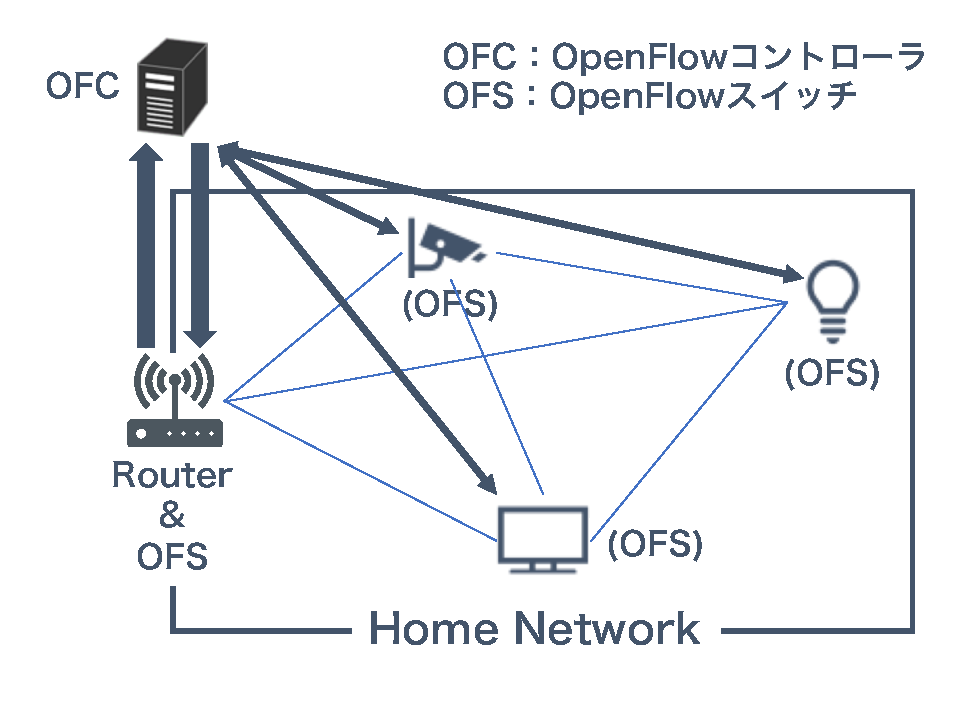
\includegraphics[width=\linewidth]{img/architecture.eps}
  \caption{提案手法の構成}
  \label{fig:architecture}
\end{figure}

%---------------------------------------------------------------------
\section{提案手法}
前述の問題点を受けて,不正アクセス拡大を防ぐことを考慮し,ホームネットワーク内においての検知も必要である.
本提案手法では,OpenFlowを利用することで,既存IoTデバイスや異なる規格などに対応でき,ホームネットワークに適した形で不正な通信の検知を実現する.
また,動的に接続を管理することで,不正通信による被害を軽減する.

\subsection{想定環境}
ホームネットワークにおける閉じたデバイス間の通信,ルーター・デバイス間の通信を想定する.
また,デバイス数は一般的に利用されているルーターの推奨接続台数である10\textasciitilde15台を想定する.

\subsection{構成}
OpenFlowを用いて,トラフィック監視を行うことで,ホームネットワーク内で行われる通信を制限する.
本提案手法の構成を図\ref{fig:architecture}に示す.
既存IoTデバイスにOpenFlowスイッチ(OFS)の機能を導入することは困難であると考え,OpenFlowスイッチの機能を持った仮想デバイスを既存IoTデバイスの前に配置する.
通信が行われる際に,仮想デバイスを通して,OpenFlowコントローラ(OFC)に接続し,トラフィック情報から通信の許可を判断する.

\subsection{動作手順}
本提案手法の動作手順のシーケンス図を図\ref{fig:sequence}に示し,詳細を以下に述べる.

\begin{enumerate}
  \item 仮想デバイス(OFS)とOFCは互いに,Echo Request/Replyメッセージを定期的に送信
  \item 接続要求デバイスは仮想デバイス(OFS)に通信
  \item 仮想デバイス(OFS)はOFCに対して,Packet Inメッセージを送信
  \item OFCはトラフィック情報を調査
  \item OFCは仮想デバイス(OFS)に対して,許可/不許可メッセージとして,Flow Modメッセージを送信
  \item OFCは仮想デバイス(OFS)に対して,Packet Outメッセージを送信
\end{enumerate}

\subsection{トラフィック情報}
本提案手法では,通信の許可を判断するトラフィック情報として,以下の3点を用いる.

\begin{itemize}
  \item パケットヘッダー
  \item パケットの長さ
  \item 周期性
\end{itemize}

%---------------------------------------------------------------------
\begin{figure}[!tb]
  \centering
  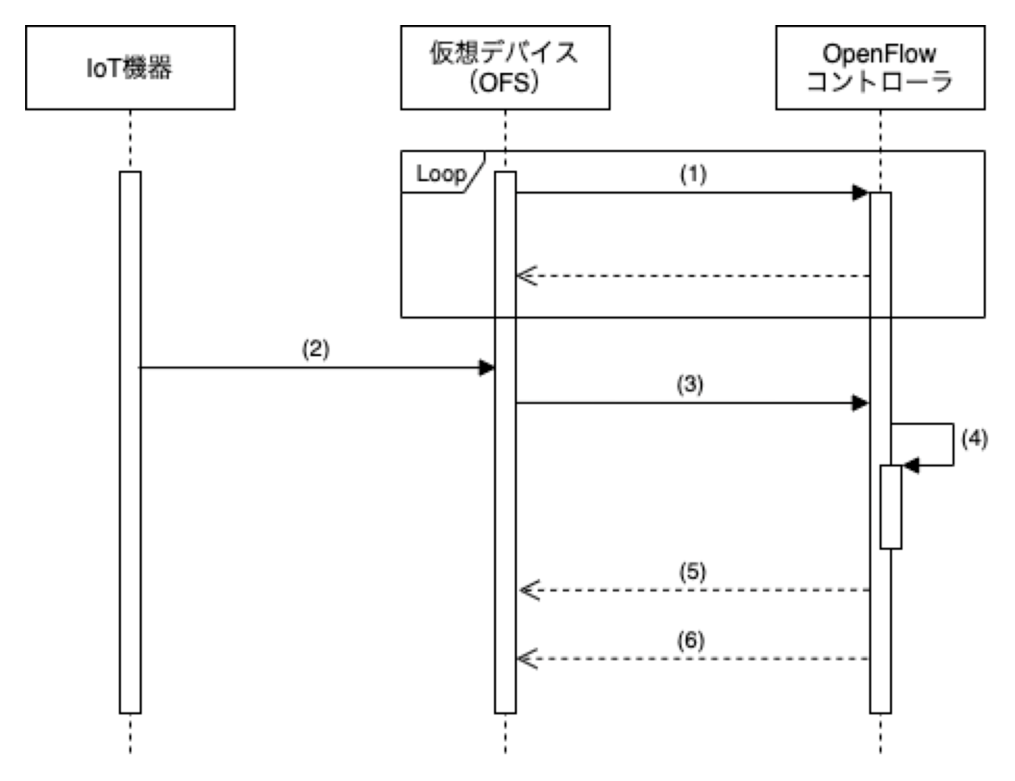
\includegraphics[width=\linewidth]{img/sequence.eps}
  \caption{動作手順のシーケンス図}
  \label{fig:sequence}
\end{figure}

%---------------------------------------------------------------------
\section{評価}
\subsection{評価項目}
本研究では,セキュリティと負荷を評価する.セキュリティ面では,正当なアクセスは通信が許可されるか,不正なアクセスは通信が許可されないかを実証する.
また,負荷面では,ネットワークに与える影響を測定したいため,スループットを評価する.

\subsection{評価シナリオ}
評価シナリオとしては,IoTデバイスが1対1,1対N,N対N($2\leqq N \leqq 15$)で通信を行っている状況を想定し,各状況において評価を行う.

%---------------------------------------------------------------------
\section{まとめ・今後の課題}
本稿では,ホームネットワークの形態の多様化からセキュリティ上の課題として,近年,増加傾向が見られる不正アクセスに着目した.
また,今後のスマートホームデバイスは,ホームネットワーク内で閉じたデバイス間の通信によって連携を行う形になることが想定される.
そこで本研究ではその対策として,OpenFlowを用いてホームネットワーク内で動的なトラフィック監視を行い,デバイス間通信における不正アクセスによる被害を軽減する手法を提案した.
本提案手法では,デバイスの前にOpenFlowスイッチの機能を持った仮想デバイスを配置し,トラフィック情報をOpenFlowコントローラで管理することで,不正アクセスを防ぐ.
\par
今後の課題としては,トラフィック情報の監視において,何を正当とし,何を不正とするのかの判断と,具体的な検知手法を検討する必要がある.
また,本提案手法の評価において,セキュリティ面の評価が重要であると考える.
評価として,正当アクセスと不正アクセスをどれほど正確に判別できるか定性的な評価を行い,セキュリティの観点からの本提案方式の有用性を示したい.

%---------------------------------------------------------------------
% Bibliography
\footnotesize{
  \begin{thebibliography}{99}
    \bibitem{guideline} IoT推進コンソーシアム, 総務省, 経済産業省, "IoTセキュリティガイドライン ver 1.0", 2016.
    \bibitem{related} 村上萌, 中村嘉隆, 高橋修, "OpenFlowを用いたホームネットワークへの接続端末制御による不正アクセス防御手法の提案", 研究報告コンピュータセキュリティ(CSEC), Vol.2016-CSEC-72, No.29, pp.1-6, 2016.
    \bibitem{d2d} C. Vallati, A. Virdis, E. Mingozzi and G. Stea, "Mobile-Edge Computing Come Home Connecting things in future smart homes using LTE device-to-device communications", IEEE Consumer Electronics Magazine, Vol.5, No.4, pp.77-83, 2016.
    \bibitem{disap} M. Serror, M. Henze, S. Hack, M. Schuba, and K. Wehrle, "Towards In-Network Security for Smart Homes", Proceedings of the 13th International Conference on Availability, Reliability and Security (ARES 2018), No.18, pp.1-8, 2018.
  \end{thebibliography}
}

%---------------------------------------------------------------------
\end{document}
%---------------------------------------------------------------------
